\documentclass[10pt,openright,twoside,french]{book}

\input philippe2013
\input philippe2013_cours
\input philippe2013_sections
\input philippe2013_chapitre
\renewcommand\PartProgramme{Stats/Probas}
\renewcommand\MaCouleur{Purple}

\pieddepage{}{%
\begin{tikzpicture}[scale=0.65]
\shadedraw [top color=white, bottom color=\MaCouleur, draw=\MaCouleur]
[l-system={Sierpinski triangle, step=1pt, angle=60, axiom=F, order=6.5}]
lindenmayer system -- cycle;
\draw (30:0.65cm) node {\bfseries\textcolor{black}{\thepage}};
\end{tikzpicture}%
}{}


\begin{document}
\chapter{Statistiques descriptives}\label{ch_stats}

\section{Vocabulaire}

Une \textbf{étude statistique} a pour but d'obtenir une information, appelée \textbf{caractère}, sur une population à partir de \textbf{données} recueillies sur un \textbf{échantillon} de cette population.

\begin{Defi}
    Le \iptb{caractère}\index{caractère!les différents types de} étudié peut être :
    \begin{description}
        \item[quantitatif :] les valeurs du caractère s'expriment avec des nombres (ex : températures, pointures, salaires\ldots) ;
        \item[qualitatif :] les valeurs ne s'expriment pas par des nombres (ex : couleurs, type d'essence\ldots) ;
        \item[discret :] les valeurs du caractère sont isolés (ex : notes\ldots) ;
        \item[continu :] les valeurs sont regroupées par classes (ou intervalles de nombre) (par ex : durée, distance parcourue,
    \end{description}
\end{Defi}

\begin{Rmq}
    Dans la suite du cours, on considère que le caractère est quantitatif.
\end{Rmq}

\begin{Defi}
    Lorsque les valeurs d'une série statistique sont regroupés par classe de type $\intervallefo a b$, on appelle \ipt{centre de classe} le nombre défini par $\frac{a + b}{2}$.
\end{Defi}

\section{Indicateurs de position}
\subsection{Moyenne}
\begin{Defi}
On considère une série qui possède des valeurs différentes $x_1, x_2, \ldots, x_p$ chacune affectée de leur effectif. L'effectif total est égal à $N$.\par
On appelle \ipt{moyenne} d'une série le nombre $\overline{m}$ tel que :
\[\overline{m} = \frac{n_1x_1 + n_2x_2 + n_3x_3 + \cdots + n_px_p}{n_1 + n_2 + \cdots + n_p} = \frac{\displaystyle\sum_{i =1}^{p}n_ix_i}{N}.\]
\end{Defi}

\begin{Exemple}
    Un élève souhaite calculer la moyennes de ses notes sur $20$ : $8 \pv 10 \pv 14 \pv 13 \pv 10 \pv 14 \pv 10$.\par\medskip
    $\overline m = \frac{8 + 10 + 14 + 13 + 10 + 14 + 10}{7} = \frac{79}{7} \approx 11,29$.\medskip

    Parfois, les valeurs sont regroupées dans un tableau : \quad
    \begin{tabular}{*{5}{|c}|}
    \hline
        Notes & $8$ & $10$ & $13$ & $14$ \\
    \hline
        Effectifs & $1$ & $3$ & $1$ & $2$ \\
    \hline
    \end{tabular}\par\medskip
    On peut alors utiliser la formule : $\overline m = \frac{1 \times 8 + 3 \times 10 + 1 \times 13 + 2 \times 14}{1 + 3 + 1 + 2} = \frac{79}{7} \approx 11,29.$
\end{Exemple}

\begin{Rmq}[s]
\begin{enumerate}
    \item En règle générale, la moyenne n'est pas une valeur de la série. On peut la considérer comme le \textnormal{point d'équilibre} des valeurs. Par conséquent, la moyenne est sensible aux valeurs extrêmes.\par
        Pour reprendre l'exemple, si la prochaine note du contrôle est très élevée alors la moyenne va augmenter.
    \item Lorsque les valeurs sont regroupés par classe, au lieu d'utiliser les $x_i$, on utilise les centres de classe.
\end{enumerate}
\end{Rmq}

\begin{Exemple}
    Le tableau ci-dessous regroupe le temps de parcours des habitants d'un village entre leur domicile et leur lieu de travail. Le maire cherche à calculer le temps moyen.
    \begin{center}
    \renewcommand\arraystretch{1.5}
        \begin{tabular}{*{7}{|c}|}
            \hline
                Durée en min & $[0 \pv 10[$ & $[10 \pv 20[$ & $[20 \pv 30[$ & $[30 \pv 50[$ & $[50 \pv 70[$ & Total \\
            \hline
                Effectif & $18$ & $35$ & $25$ & $112$ & $80$ & $270$ \\
            \hline
                Centre de classe & $5$ & $15$ & $25$ & $40$ & $60$ & \\
            \hline
        \end{tabular}
    \renewcommand\arraystretch{1}
    \end{center}
    On a donc : $\overline m = \frac{18 \times 5 + 35 \times 15 + 25 \times 25 + 112 \times 40 + 80 \times 60}{270} = \frac{\NP{10520}}{270} \approx 39~min.$
\end{Exemple}

\subsection{Médiane}

\begin{Defi}
    On considère une série statistique dont l'effectif total est égal à $N$. Les valeurs sont rangées dans l'ordre croissant.

    \textbf{Une} \ipt{médiane} $Me$ est un nombre réel qui permet de partager la série statistique en deux séries de même valeur.

    Autrement dit, la moitié ($50\%$) des valeurs de la série est inférieure ou égale à $Me$ et l'autre moitié est supérieure ou égale à $Me$.

\begin{center}
    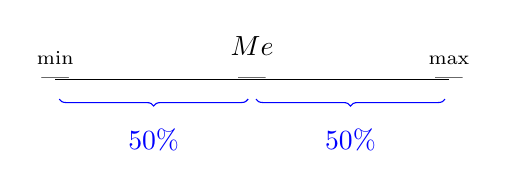
\begin{tikzpicture}
        \draw (0,0)--(5,0) node[midway] {|} node[midway,above=5pt] {$Me$};
        \draw (0,0) node {|} node[above=2pt] {\scriptsize $\min$}; \draw (5,0) node {|} node[above=2pt] {\scriptsize $\max$};
        \draw[color=blue,decorate,decoration={brace,raise=0.25cm}] (2.45,0) -- (0.05,0) node[below=0.5cm,pos=0.5] {$50\%$};
        \draw[color=blue,decorate,decoration={brace,raise=0.25cm}] (4.95,0) -- (2.55,0) node[below=0.5cm,pos=0.5] {$50\%$};
    \end{tikzpicture}
\end{center}
\end{Defi}

\textbf{Méthode de calcul :} Par définition, la médiane dépend de l'effectif de la série :
\begin{itemize}
    \item Si $N$ est impair, alors on calcule $\frac{N + 1}{2}$ et le résultat correspond à la position de la médiane choisie dans la série.
    \item Si $N$ est pair, alors la médiane choisie est égale à la moyenne de la valeur situé à la position $\frac N 2$ et la valeur suivante.
\end{itemize}

\begin{Exemple}
On considère le relevé des températures en janvier et en février dans une ville :
\begin{center}
\renewcommand\arraystretch{1.5}
    \begin{tabular}{*{10}{|c}|}
        \hline
            \multicolumn{10}{|c|}{Janvier}\\
        \hline
            Valeurs & $-3\degres$ & $-2\degres$ & $-1\degres$ & $0\degres$ & $1\degres$ & $2\degres$ & $3\degres$ & $4\degres$ & Total \\
        \hline
            Effectifs & $3$ & $5$ & $8$ & $5$ & $4$ & $3$ & $2$ & $1$ & $31$\\
        \hline
            \multicolumn{10}{|c|}{Février}\\
        \hline
            Valeurs & $-3\degres$ & $-2\degres$ & $-1\degres$ & $0\degres$ & $1\degres$ & $2\degres$ & $3\degres$ & $4\degres$ & Total \\
        \hline
            Effectifs & $1$ & $2$ & $3$ & $3$ & $5$ & $9$ & $3$ & $2$ & $28$\\
            \hline
    \end{tabular}
\renewcommand\arraystretch{1}
\end{center}\medskip

\begin{description}
    \item[En janvier :] $N = 31$ donc $\frac{N+1}{2} = 16$ : une médiane possible est la $16$\ieme valeur donc $Me = -1\degres$. En janvier, il a fait moins de $-1\degres$ la moitié du mois.
    \item[En févier :] $N = 28$ donc $\frac{N}{2} = 14$ : la $14\ieme$ est $1\degres$ et la suivante est égale à $2\degres$. Donc la moyenne des deux est $\frac{1+2}{2} = 1,5$. Une médiane possible est égale à $1,5\degres$ donc durant la moitié du mois, la température a été supérieure à $1,5\degres$.
\end{description}
\end{Exemple}

\begin{Rmq}
    Contrairement à la moyenne, la médiane n'est pas sensible aux valeurs extrêmes. En effet, dans notre exemple, si la dernière température était égale à $20\degres$ au lieu de $4\degres$, la moyenne augmenterait alors que la médiane resterait identique car l'effectif total n'a pas changé.
\end{Rmq}

\subsection{Quartiles}

\begin{Defi}
    On considère une série statistique $S$ dont l'effectif total est égal à $N$. Les valeurs sont rangées dans l'ordre croissant.
    \begin{itemize}
        \item Le \ipt{premier quartile}\index{quartile} $Q_1$ de $S$ est le plus petit élément $a$ de $S$ tel qu'au moins $25\%$ des données soient inférieures ou égales à $a$.
        \item Le \ipt{troisième quartile}\index{quartile} $Q_3$ de $S$ est le plus petit élément $b$ de $S$ tel qu'au moins $75\%$ des données soient inférieures ou égales à $b$.
    \end{itemize}

\begin{center}
    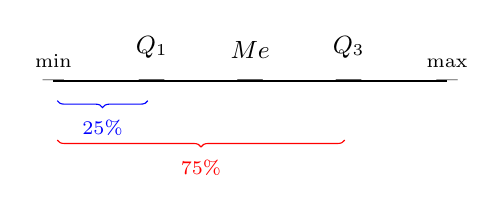
\begin{tikzpicture}
        \begin{small}
        \draw (0,0)--(5,0) node[midway] {|} node[midway,above=5pt] {$Me$} node[pos=0.75,above=5pt] {$Q_3$} node[pos=0.25,above=5pt] {$Q_1$};
        \draw (0,0)--(5,0) node[pos=0.25] {|}; \draw (0,0)--(5,0) node[pos=0.75] {|};
        \end{small}
        \begin{scriptsize}
        \draw (0,0) node {|} node[above=2pt] {$\min$}; \draw (5,0) node {|} node[above=2pt] {$\max$};
        \draw[color=blue,decorate,decoration={brace,raise=0.25cm}] (1.2,0) -- (0.05,0) node[below=0.4cm,pos=0.5] {$25\%$};
        \draw[color=red,decorate,decoration={brace,raise=0.75cm}] (3.7,0) -- (0.05,0) node[below=0.9cm,pos=0.5] {$75\%$};
        \end{scriptsize}
    \end{tikzpicture}
\end{center}
\end{Defi}

\textbf{Méthode de calcul :} Par définition, les quartiles dépendent de l'effectif de la série :
\begin{description}
    \item[Premier quartile :] On arrondit le nombre $\frac{N}{4}$ à l'unité par excès et cela donne la position de $Q_1$ dans la série $S$.
    \item[Troisième quartile :] On arrondit le nombre $3\times\frac{N}{4}$ à l'unité par excès et cela donne la position de $Q_3$ dans la série $S$.
\end{description}

\begin{Exemple}
    On reprend les températures du moins de janvier de l'exemple précédent.
    \begin{description}
        \item[Premier quartile :] $N = 31$ donc $\frac N 4 = 7,75 \approx 8$ donc la $8\ieme$ valeur est $Q_1 = -2\degres$.
        \item[Troisième quartile :] $N = 31$ donc $3\times\frac N 4 = 23,25 \approx 24$ donc la $24\ieme$ valeur donne $Q_3 = 1\degres$.
    \end{description}
    Ainsi, $25\%$ des valeurs sont inférieures ou égales à $-2\degres$ et $75\%$ des valeurs sont inférieures ou égales à $1\degres$. On peut dire aussi que $25\%$ des valeurs sont supérieures ou égales à $1\degres$.
\end{Exemple}

\section{Indicateurs de dispersion}

Dans les classes antérieures, l'\iptb{étendue} était un indicateur de dispersion utilisé dont voici rappelée la définition :

\begin{Defi}
    Dans une série statistique, l'\iptb{étendue}\index{etendue@étendue} est la différence entre la valeur maximale et la valeur minimale.
\end{Defi}

\begin{Rmq}
    Une valeur élevée de l'étendue signifie qu'au moins une des valeurs extrêmes de la série est éloignée de la médiane et le risque de dispersion des valeurs est donc plus important.\par
    Dans l'exemple précédent, l'étendue de la série \textnormal{janvier} était identique à celle de la série \textnormal{février} ce qui montre les besoins d'avoir d'autres indicateurs.\par
    Les quartiles nous permettent d'obtenir d'autres indicateurs de dispersion lié à la médiane.
\end{Rmq}

\subsection{Intervalle et écart interquartile}

\begin{Defi}
    On appelle l'\ipt{intervalle interquartile} l'intervalle $\intervalleff{Q_1}{Q_3}$.\par
    On appelle l'\iptb{écart interquartile}\index{ecart interquartile@écart interquartile} le nombre $Q_3 - Q_1$.
\end{Defi}

\begin{Rmq}
\begin{center}
    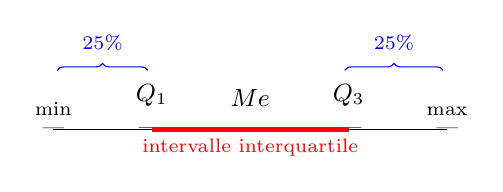
\begin{tikzpicture}
        \begin{small}
        \draw (0,0)--(5,0) node[midway] {|} node[midway,above=5pt] {$Me$} node[pos=0.75,above=5pt] {$Q_3$} node[pos=0.25,above=5pt] {$Q_1$};
        \draw (0,0)--(5,0) node[pos=0.25] {|}; \draw (0,0)--(5,0) node[pos=0.75] {|};
        \end{small}
        \begin{scriptsize}
        \draw (0,0) node {|} node[above=2pt] {$\min$}; \draw (5,0) node {|} node[above=2pt] {$\max$};
        \draw[color=blue,decorate,decoration={brace,raise=0.75cm}] (0.05,0) -- (1.2,0) node[above=0.9cm,pos=0.5] {$25\%$};
        \draw[color=blue,decorate,decoration={brace,raise=0.75cm}] (3.7,0) -- (4.95,0) node[above=0.9cm,pos=0.5] {$25\%$};
        \draw[red,line width=2pt] (1.25,0)--(3.75,0) node[midway,below] {intervalle interquartile};
        \end{scriptsize}
    \end{tikzpicture}
\end{center}

La figure ci-dessus nous permet de comprendre pourquoi l'intervalle interquartile contient $50\%$ de valeurs de la série, c'est-à-dire la moitié. Ainsi, un écart interquartile faible impose que les valeurs soient regroupées proches de la médiane et donc peu dispersée pour la moitié d'entre elles.
\end{Rmq}

\subsection{Variance et écart-type}
On s'intéresse ici à l'écart existant entre chaque valeur de la série et la moyenne. Puis on calcule la moyenne de ces écarts. Dans ce cas, on trouve $0$. En effet :
\[\begin{split}
    \frac{x_1 - \overline m + x_2 - \overline m + \cdots + x_n - \overline m}{n} &= \frac{x_1 + x_2 + \cdots x_n}{n} - \frac{n \times \overline m}{n} \\
    &= \overline m - \overline m \\
    &= 0
\end{split}\]

Pour éviter ce résultat, on utilise la même méthode mais en calculant la moyenne des carrés des écarts.

\begin{Defi}
    Soit $S$ une série statistique de valeurs $x_1$, $x_2, \ldots, x_n$ et de moyenne $\overline m$. La \ipt{variance} est le nombre positif ou nul $V$ défini par :
    \[V = \frac{(x_1 - \overline m)^2 + (x_2 - \overline m)^2 + \cdots + (x_3 - \overline m)^2}{n} = \frac1n \sum_{i = 1}^{n}(x_i - \overline m)^2.\]
\end{Defi}

\begin{Exemple}
    Prenons une série de notes :
    \begin{center}
    \renewcommand\arraystretch{2}
        \begin{tabular}{|c|*{6}{m{1.5cm}|}}
            \hline
                Notes & $7$ & $9$ & $12$ & $13$ & $15$ & $18$ \\
            \hline
                Effectifs & $1$ & $2$ & $1$ & $2$ & $4$ & $2$ \\
            \hline
                \multicolumn{7}{|c|}{Moyenne : $\overline m = 159 \div 12 = 13,25$} \\
            \hline
                $(x_i - \overline m)$ & $-6,25$ & $-4,25$ & $-1,25$ & $-0,25$ & $1,75$ & $4,75$ \\
            \hline
                $(x_i - \overline m)^2$  & $39,0625$  & $18,0625$ & $1,5625$ &$0,0625$ & $3,0625$ & $22,5625$  \\
            \hline
                \multicolumn{7}{|c|}{Variance : $V = (39,0625 \times 1 + 18,0625 \times 2 + \cdots + 22,5625 \times 2) \div 12 = 134,25 \div 12 = 11,1875$} \\
            \hline
        \end{tabular}
    \renewcommand\arraystretch{1}
    \end{center}
    La moyenne des carrés des écarts est donc égale à $11,1875$.
\end{Exemple}

\begin{Thm}[de König-Huygens (admis)]
    Soit $S$ une série statistique de valeurs $x_1$, $x_2, \ldots, x_n$ et de moyenne $\overline m$.\par
    On pose $\overline n = \frac{x_1^2 + x_2^2 + \cdots + x_n^2}{n}$ (moyenne des carrés des valeurs).\par
    La variance $V$ de la série statistique est alors égale à :
    \[V = \overline n - (\overline m)^2.\]
\end{Thm}\clearpage

\begin{Exemple}
    Avec l'exemple précédent :
    \begin{center}
    \renewcommand\arraystretch{2}
        \begin{tabular}{|c|*{6}{m{1.5cm}|}}
            \hline
                Notes & $7$ & $9$ & $12$ & $13$ & $15$ & $18$ \\
            \hline
                Effectifs & $1$ & $2$ & $1$ & $2$ & $4$ & $2$ \\
            \hline
                \multicolumn{7}{|c|}{Moyenne : $\overline m = 159 \div 12 = 13,25$} \\
                \multicolumn{7}{|c|}{donc $(\overline m)^2 = 175,5625$} \\
            \hline
                $(x_i)^2$ & $49$ & $81$ & $144$ & $169$ & $225$ & $324$ \\
            \hline
                \multicolumn{7}{|c|}{Moyenne des carrés : $\overline n = \NP{2241} \div 12 = 186,75$} \\
            \hline
                \multicolumn{7}{|c|}{Variance : $V = 186,75 - 175,5625 = 11,1875$} \\
            \hline
        \end{tabular}
    \renewcommand\arraystretch{1}
    \end{center}
    On trouve bien le même résultat mais en faisant intervenir la moyenne qu'une seule fois.
\end{Exemple}\medskip

Cela n'est cependant pas exploitable car l'unité de mesure n'est plus la même depuis que l'on a utilisé des nombres au carré. On s'intéresse donc surtout à l'indicateur suivant :\medskip

\begin{Defi}
    Soit $S$ une série statistique de variance $V$. L'\iptb{écart-type}\index{ecart-type@écart-type} $\sigma$ est le nombre réel positif défini par : \[\sigma = \sqrt V.\]
\end{Defi}

\begin{Rmq}
    L'écart-type est un nombre réel positif qui caractérise la dispersion des valeurs d'une série statistiques par rapport à la moyenne.\par
    Plus l'écart-type est petit et plus les valeurs sont proches de la moyenne (dispersion faible). Au contraire, si l'écart-type est grand alors les valeurs sont éloignés de la moyenne (dispersion élevée).\par
    Calculer l'écart-type est notamment intéressant pour comparer plusieurs séries statistiques dont les valeurs sont exprimées dans la même unité de mesure.
\end{Rmq}\medskip

\begin{Exemple}
    Dans l'exemple précédent, on obtient $\sigma = \sqrt{11,1875} \approx 3,34$.\par
    Cela donne une indication de la répartition moyenne des notes autour de la moyenne $\overline m$.
\end{Exemple}

\begin{Rmq}
    En \premiere\sti, on utilisera la plupart du temps la calculatrice ou le tableur pour calculer directement la variance et l'écart-type.\par
    On se servira alors des fonctions \bsc{\texttt{var.p}} et \bsc{\texttt{ecartypep}} ou encore, pour la dernière version de \bsc{\texttt{Excel}} : \bsc{\texttt{var.p.n}} et \bsc{\texttt{ecartype.pearson}}
\end{Rmq}



\end{document}
